\fuxiti
\begin{xiaotis}
\begin{enhancedline}

\xiaoti{$\triangle ABC$ 中, $AB = AC$, $AD$ 为 $BC$ 边上的高, $AD$ 的中点为 $M$,
    $CM$ 的延长线交 $AB$ 于点 $K$。 求证: $AB = 3AK$。
}

\xiaoti{已知: $\triangle ABC$ 中, $AB = 15$, $AC = 20$, 高 $AD = 12$。求角平分线 $AE$ 的长。}

\xiaoti{$O$ 为四边形 $ABCD$ 的对角线 $AC$ 的中点。 $OE$、$OF$、$OG$、$OH$ 分别是
    $\angle AOB$、$\angle BOC$、$\angle COD$、$\angle DOA$ 的平分线,
    且分別和 $AB$、$BC$、$CD$、$DA$ 交于点 $E$、$F$、$G$、$H$。
    求证: $EF \pingxing GH$。
}

\xiaoti{$\triangle ABC$ 中,角平分线 $AD$、$BE$ 交于点 $I$。
    求证; $\dfrac{AI}{ID} = \dfrac{AB + AC}{BC}$。
}

\xiaoti{$\pxsbx ABCD$ 中, $\angle DAB$ 的平分线交 $BD$ 于点 $P$。
    $\angle ADC$ 的平分线交 $CA$ 于点 $Q$。 求证: $PQ \pingxing DA$。
}

\xiaoti{射击瞄准时,要求枪的标尺缺口上沿中央 $A$、准星尖 $B$ 和瞄准点 $C$ 在一条直线上(上图),这样才能命中目标。
    已知某种冲锋枪基线 $AB$ 长 $38.5\;\limi$(下图),如果射击距离  $AC = 100\;\mi$,
    当准星尖在缺口内偏差 $BB'$ 为 $1\;\haomi$ 时,弹着偏差 $CC'$ 是多少( $BB' \pingxing CC'$)?
}

\begin{figure}[htbp]
    \centering
    \begin{minipage}[b]{7cm}
        \centering
        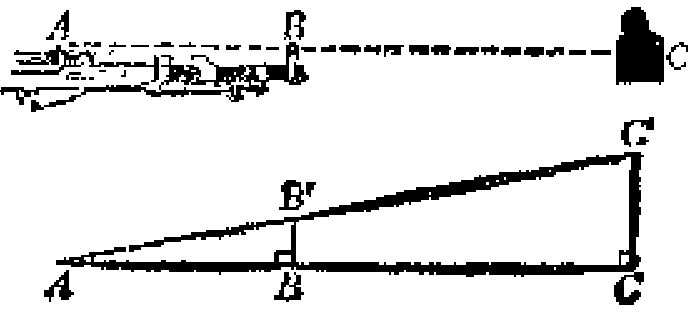
\includegraphics[width=6cm]{../pic/czjh2-ch6-fuxi-06.png}
        \caption*{(第 6 题)}
    \end{minipage}
    \qquad
    \begin{minipage}[b]{7cm}
        \centering
        \begin{tikzpicture}
    \tkzDefPoints{0/0/B, 2/0/C, 0.4/2/A}
    \tkzInterLC[R, near](A,B)(B,1.5)  \tkzGetFirstPoint{D}
    \tkzInterLC[R, near](A,C)(C,1.5)  \tkzGetFirstPoint{E}
    \tkzInterLL(D,E)(B,C)  \tkzGetPoint{F}

    \tkzDrawPolygon(A,B,C)
    \tkzDrawSegments(D,F  C,F)
    \tkzLabelPoints[above](A)
    \tkzLabelPoints[above,xshift=.3em](E)
    \tkzLabelPoints[left](B,D)
    \tkzLabelPoints[below](C)
    \tkzLabelPoints[right](F)
\end{tikzpicture}


        \caption*{(第 10 题)}
    \end{minipage}
\end{figure}


\xiaoti{在 $\triangle ABC$($AB > AC$)的边 $AB$ 上取一点 $D$, 在边 $AC$ 上取一点 $E$,
    使 $AD = AE$, 直线 $DE$ 和 $BC$ 的延长线交于点 $P$。
    求证: $BP:CP = BD:CE$。(提示:经过点 $C$ 作 $AB$ 的平行线。)
}

\xiaoti{已知: $\triangle ABC$ 中,中线 $BE$ 与角平分线 $AD$ 交于点 $K$, $BL \pingxing KC$,
    交 $AC$ 的延长线于点 $L$。求证:$LC = AB$。
}

\xiaoti{过 $\triangle ABC$ 的顶点 $C$ 任作一直线, 与边 $AB$ 及中线 $AD$ 分别交于点 $F$ 及 $E$。\\
    求证: $AE:ED = 2 AF:FB$。
}

\xiaoti{如图, $BD = CE$。 求证: $AC \cdot EF = AB \cdot DF$。}

\xiaoti{一直线和梯形 $ABCD$ 的底 $AD$ 平行,和 $AB$、$BD$、$AC$、$CD$ 分别交于点 $E$、$F$、$G$、$H$。求证: $EF = GH$。}

\xiaoti{$Rt \triangle ABC$ 中有正方形 $DEFG$,点 $D$、$G$ 分别在 $AB$、$AC$ 上,$EF$ 在斜边 $BC$ 上。求证:$EF^2 = BE \cdot FC$。}

\xiaoti{已知:如图,$\triangle PQR$ 是等边三角形,$\angle APB = 120^\circ$。求证:}
\begin{xiaoxiaotis}

    \xxt{$\triangle PAQ \xiangsi \triangle BPR$;}

    \xxt{$AQ \cdot RB = QR^2$。}

\end{xiaoxiaotis}

\begin{figure}[htbp]
    \centering
    \begin{minipage}[b]{7cm}
        \centering
        \begin{tikzpicture}
    \tkzDefPoints{0/0/Q, 2/0/R}
    \tkzDefTriangle[equilateral](Q,R)  \tkzGetPoint{P}
    \tkzDefTriangle[two angles=120 and 20](Q,P)  \tkzGetPoint{A}
    \tkzDefTriangle[two angles=35 and 120](P,R)  \tkzGetPoint{B}

    \tkzDrawPolygon(P,Q,R)
    \tkzDrawPolygon(A,P,Q)
    \tkzDrawPolygon(B,P,Q)
    \tkzLabelPoints[above](P)
    \tkzLabelPoints[left](A)
    \tkzLabelPoints[right](B)
    \tkzLabelPoints[below](Q,R)
\end{tikzpicture}


        \caption*{(第 13 题)}
    \end{minipage}
    \qquad
    \begin{minipage}[b]{7cm}
        \centering
        \begin{tikzpicture}
    \tkzDefPoints{0/0/D, 2/0/C}
    \tkzDefTriangle[two angles=105 and 40](D,C)  \tkzGetPoint{A}
    \tkzDefTriangle[two angles=75  and 40](D,A)  \tkzGetPoint{B}
    \tkzDefLine[bisector](D,A,C)  \tkzGetPoint{e}
    \tkzInterLL(A,e)(D,C)  \tkzGetPoint{E}

    \tkzDrawPolygon(A,B,C)
    \tkzDrawSegments(A,D  A,E)
    \tkzLabelPoints[above](A)
    \tkzLabelPoints[left](B)
    \tkzLabelPoints[right](C)
    \tkzLabelPoints[below](D,E)
\end{tikzpicture}


        \caption*{(第 14 题)}
    \end{minipage}
\end{figure}

\xiaoti{已知:$D$、$E$ 是 $\triangle ABC$ 的边 $BC$ 上的两点,且 $\angle BAD = \angle C$,
    $\angle DAE = \angle EAC$。求证: $\dfrac{BD}{BA} = \dfrac{DE}{EC}$。
}

\xiaoti{$AD$ 为 $\triangle ABC$($AB > AC$)的角平分线, $AD$ 的垂直平分线和 $BC$ 的延长线交于点 $E$。
    求证:$DE^2 = BE \cdot CE$。
}

\xiaoti{已知:$\triangle ABC$ 中, $\angle C$ 是直角, $CD$ 是高, $AE$ 是角平分线。
    求证:$\dfrac{CE}{EB} = \dfrac{CD}{CB}$。
}

\xiaoti{已知:$\triangle ABC$, $AD$ 是高,且 $AD^2 = BD \cdot CD$。
    求证: $\angle BAC = 90^\circ$。
}

\xiaoti{$AH$,$A'H'$ 分别是两锐角三角形 $\triangle ABC$ 与 $\triangle A'B'C'$ 的高,
    并且  $\dfrac{AB}{A'B'} = \dfrac{BC}{B'C'} = \dfrac{AH}{A'H'}$。
    求证: $\triangle ABC \xiangsi \triangle A'B'C'$。
}

\xiaoti{$AD$、$A'D'$ 分别是 $\triangle ABC$ 和 $\triangle A'B'C'$ 的角平分线,
    并且 $\dfrac{AB}{A'B'} = \dfrac{BD}{B'D'} = \dfrac{AD}{A'D'}$。
    求证: $\triangle ABC \xiangsi \triangle A'B'C'$。
}

\xiaoti{已知:如图, $\triangle ABC$ 中, $DE \pingxing BC$, $BE$ 与 $CD$ 于点 $O$,
    $AO$ 与 $DE$、$BC$ 分别交于点 $N$、$M$。
    求证: $\dfrac{AN}{AM} = \dfrac{ON}{OM}$。
}

\begin{figure}[htbp]
    \centering
    \begin{minipage}[b]{7cm}
        \centering
        \begin{tikzpicture}
    \tkzDefPoints{0/0/B, 4/0/C, 1.7/2.5/A}
    \tkzDefPointOnLine[pos=0.4](A,B)  \tkzGetPoint{D}
    \tkzDefPointOnLine[pos=0.4](A,C)  \tkzGetPoint{E}
    \tkzInterLL(B,E)(C,D)  \tkzGetPoint{O}
    \tkzInterLL(A,O)(B,C)  \tkzGetPoint{M}
    \tkzInterLL(A,O)(D,E)  \tkzGetPoint{N}

    \tkzDrawPolygon(A,B,C)
    \tkzDrawSegments(B,E  C,D  D,E  A,M)
    \tkzLabelPoints[above](A)
    \tkzLabelPoints[left](B,D)
    \tkzLabelPoints[right](C,E)
    \tkzLabelPoints[below](M)
    \tkzLabelPoints[above,xshift=.4em](N)
    \tkzLabelPoints[below,xshift=-.4em](O)
\end{tikzpicture}


        \caption*{(第 20 题)}
    \end{minipage}
    \qquad
    \begin{minipage}[b]{7cm}
        \centering
        \begin{tikzpicture}
    \pgfmathsetmacro{\a}{1.5}
    \tkzDefPoints{0/0/B, \a/0/E, 2*\a/0/F, 3*\a/0/C}
    \tkzDefPoints{0/\a/A, \a/\a/G, 2*\a/\a/H, 3*\a/\a/D}

    \tkzDrawPolygon(A,B,C,D)
    \tkzDrawSegments(G,E H,F A,E A,F A,C)
    \tkzLabelPoints[left](A,B)
    \tkzLabelPoints[right](C,D)
    \tkzLabelPoints[above](G,H)
    \tkzLabelPoints[below](E,F)
\end{tikzpicture}


        \caption*{(第 21 题)}
    \end{minipage}
\end{figure}

\xiaoti{如图,四边形 $ABEG$、$GEFH$、$HFCD$ 都是边长为 $a$ 的正方形。}
\begin{xiaoxiaotis}

    \xxt{计算 $AE$、$AF$、$AC$ 的长;}

    \xxt{求证:$\triangle AEF \xiangsi \triangle CEA$;}

    \xxt{求证:$\angle AFB + \angle ACB = 45^\circ$。}

\end{xiaoxiaotis}


\xiaoti{$\triangle ABC$ 与 $\triangle DEF$ 中, $\angle A = \angle D$,$\angle B = \angle E$,
    $AB = EF$, $BC = DF$, 这两个三角形相似吗?全等吗?设 $AB = 1$, $BC = 1.1$,
    找出符合条件的两个三角形的边长。
}

\xiaoti{\footnotemark 如图,正方形城邑 $DEFG$ 的四面正中各有城门,出北门 20 步的 $A$ 处($HA = 20$ 步)有一树木,
    出南门 14 步到 $C$ 处($KC = 14$ 步), 再向西行 1775 步到B处($CB = 1775$ 步),
    正好看到 $A$ 处的树木(点 $D$ 在直线 $AB$ 上)。求城邑的边长 $x$($FG = x$)。
}
\footnotetext{本题是我国古代数学书《九章算术》中“勾股”章的第二十题。
    原文是:“今有邑不知大小,各中开门,出北门二十步有木,
    出南门十四步折而西行一千七百七十五步见木,问邑方几何。”
}

\begin{figure}[htbp]
    \centering
    \begin{minipage}[b]{7cm}
        \centering
        \begin{tikzpicture} % 本图线段不成比例,仅供参考示意
    \pgfmathsetmacro{\a}{1.5}
    \tkzDefPoints{0/0/E, \a/0/F, \a/\a/G, 0/\a/D}
    \tkzDefMidPoint(D,G)  \tkzGetPoint{H}
    \tkzDefMidPoint(E,F)  \tkzGetPoint{K}
    \tkzDefShiftPoint[H](0,0.5){A}
    \tkzDefShiftPoint[K](0,-0.4){C}
    \tkzDefShiftPoint[C](-0.1,0){b}
    \tkzInterLL(A,D)(C,b)  \tkzGetPoint{B}

    \tkzDrawPolygon[pattern={mylines[angle=45, distance={4pt}]}](E,F,G,D)
    \tkzDrawPolygon(A,B,C)
    \tkzLabelPoints[above](A)
    \tkzLabelPoints[left](B,D,E)
    \tkzLabelPoints[below](C)
    \tkzLabelPoints[right](F,G)
    \tkzLabelPoints[above right](H)
    \tkzLabelPoints[below right](K)
\end{tikzpicture}


        \caption*{(第 23 题)}
    \end{minipage}
    \qquad
    \begin{minipage}[b]{7cm}
        \centering
        \begin{tikzpicture} % 本图线段不成比例,仅供参考示意
    \tkzDefPoints{0/0/B, 0/2/A, 1.5/0/D, 1.5/0.5/C, 3.5/0/F, 3.5/0.5/E}
    \tkzInterLL(A,C)(B,D)  \tkzGetPoint{G}
    \tkzInterLL(A,E)(B,D)  \tkzGetPoint{H}
    \tkzInterLL(E,C)(A,B)  \tkzGetPoint{K}

    \tkzDrawSegments(A,B  C,D  E,F A,G  A,H B,H)
    \tkzDrawSegment[dashed](E,K)
    \tkzLabelPoints[above](A)
    \tkzLabelPoints[left](B,K)
    \tkzLabelPoints[below](D,G,F)
    \tkzLabelPoints[right](H)
    \tkzLabelPoints[above,xshift=.3em](C,E)
\end{tikzpicture}


        \caption*{(第 24 题)}
    \end{minipage}
\end{figure}

\xiaoti{\footnotemark 为了求出海岛上的山峰 $AB$ 的高度, 在 $D$ 和 $F$ 处树立标杆 $DC$ 和 $FE$,
    标杆的高都是 3 丈,相隔 1000 步( 1 步等于 5 尺),并且 $AB$、$CD$ 和 $EF$ 在同一平面内,
    从标杆 $DC$ 退后 123 步的 $G$ 处,可看到山峰 $A$ 和标杆顶端 $C$ 在一直线上;
    从标杆 $FE$ 退后 127 步的 $H$ 处,可看到山峰 $A$ 和标杆顶端 $E$ 在一直线上。
    求山峰的高度 $AB$ 及它和标杆 $CD$ 的水平距离 $BD$ 各是多少?\\
    (提示:连结 $EC$ 井延长交 $AB$ 于点 $K$, 用 $AK$ 表示 $KC$ 及 $KE$。)
}
\footnotetext{本题是我国魏晋时数学家刘徽所著《海岛算经》中九个代表性数学问题的第一题。
    原文是:“今有望海岛,立两表齐高三丈,前后相去千步,今后表与前表参相直,
    从前表却行一百二十三步,人目着地取望岛峰与表末参合,
    从后表却行一百二十七步,人目着地取望岛峰亦与表末参合。
    问岛高及去表各几何。”
}

\xiaoti{已知:正方形 $ABCD$, $E$ 是 $AB$ 的中点, $F$ 是 $AD$ 上的一点,
    且 $AF = \exdfrac{1}{4} AD$,$EG \perp CF$, 垂足为 $G$。
    求证: $EG^2 = CG \cdot FG$。
}

\begin{withstar}
\xiaoti{作一个等边三角形,使它的三个顶点分別在 $\triangle ABC$ 的三边上,
    并且有一边和 $BC$ 平行。
}
\end{withstar}

\end{enhancedline}
\end{xiaotis}

